\section{Introduction}

With the rapid development of medical big data, forecasting future or potential diseases based on patients' past medical records has emerged as a promising approach towards preventing high-risk diseases.
Rather than individualizing patients (e.g., via screening or counseling), a medical informatics system can predict each patient's potential diseases using his or her past diagnoses as well as diagnoses collected from many other patients.
In this way, the medical system can identify high-risk patients from a large corpus of patients with low cost.
These high-risk patients can then receive targeted care to employ disease prevention techniques in advance.
Naturally, the accuracy of such early disease detection is crucial to improving the efficiency of high-risk patient identification and disease prevention. 


In this paper, we present \TheName{}---an extended linear discriminant analysis (LDA)~\cite{fisher1936use,mclachlan2004discriminant} framework for early disease detection using Electronic Health Records (EHR), which can improve the prediction accuracy of the standard LDA model by reducing noise in EHR data and regularizing the estimated covariance matrices.
We first discuss the motivations and background of this research, then we formulate a new research problem based on our observations and assumptions.
We elaborate the technical challenges of the proposed research. 
Finally, we summarize our technical contributions.
 

\subsection{Motivations and Backgrounds}

To predict patients' potential diseases according to their past medical records, a variety of predictive models utilizing heterogeneous medical data have been studied~\cite{soni2011predictive,palaniappan2008intelligent,kumari2011comparative}.
For example, chest imaging has been used for early detection of chest cancer~\cite{FIXME}, questionnaire-based assessment (e.g., PHQ-9~\cite{kroenke2002phq}) data for predicting mental disorders, and screening data for predicting heart disease~\cite{d2001validation}.
Among these medical data, Electronic Health Records (EHR) consisting of the diagnosis records from patients' visits are used as a general purpose data source that enables early disease detection based on the previous diagnoses at a massive scale.
Furthermore, this data is more accessible to clinicians and researchers, and holds comprehensive information of patients' medical history, especially within the primary care setting.
Thus, EHR data provides a promising opportunity for early disease detection due to its generality, accessibility, and standardized use and features. 
 

As shown in Figure~\ref{fig:exp-ehr}, a patient's EHR data includes all his/her past diagnosis and treatment records, where the diagnosis record includes a sequence of visits, and each visit consists of multiple diagnoses.
Note that all diagnoses are recorded using ICD-9 codes~\cite{dubberke2006icd}, where each evidence of diagnosis corresponds to a specific ICD-9 code.
With diagnosis records in the EHR data, several methods~\cite{personalized2015, amarasingham2010automated, pittman2004integrated,jensen2012mining} have been studied to predict the disease of patients.
Given a disease as the prediction target (e.g., anxiety/depression) as well as the EHR data of a large population with or without the target disease, most existing methods first represent each given patient's EHR data using a set of features, and then train a predictive model using features and labels (if each patient is diagnosed with the targeted disease) in a supervised manner.
Further, given each new patient's EHR data, these models predict if the given patient will develop the targeted disease in near future using the trained predictive model.
 

\begin{figure}
\centering
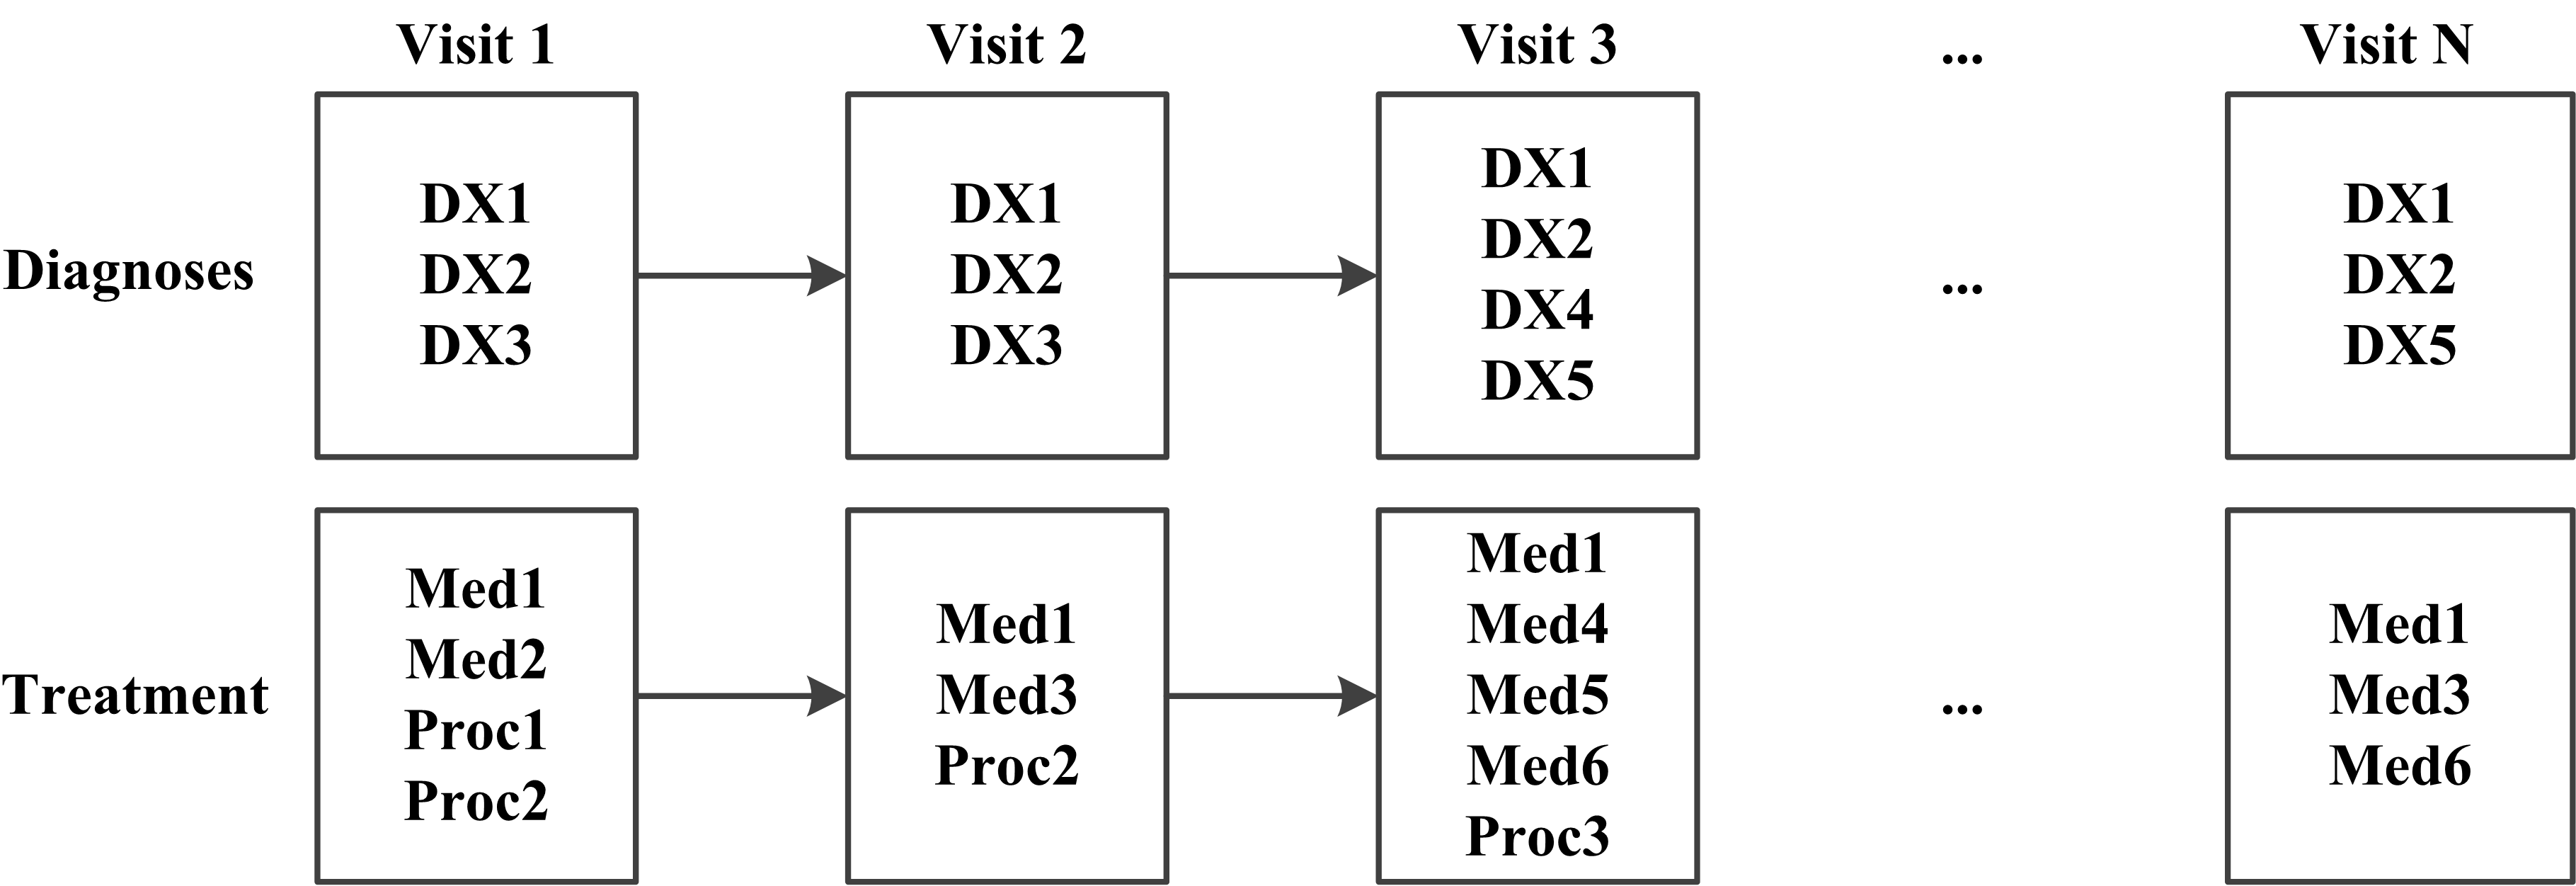
\includegraphics[width=0.48\textwidth]{./img/Patient.png}
\caption{An Example of a Patient's EHR Data}
\label{fig:exp-ehr}
\end{figure}


\textbf{EHR Data Representation for Early Detection.} 
In terms of representing EHR data, existing approaches include using diagnosis-frequencies~\cite{sun2012supervised,7091853,personalized2015}, pairwise diagnosis transitions~\cite{zhang_mseq_2015,jensen2001mining}, graph representations of diagnosis sequences~\cite{liu_temporal_2015}, and so on.
Among these approaches, the diagnosis-frequency is one common way to represent EHR data.
Given each patient's EHR data, which consists of the patient's demographic information and a sequence of past visits, existing methods first retrieve the diagnosis codes recorded during each visit.
Next, the frequency of each diagnosis appearing in all past visits are counted, followed by further transformation on the frequency of each diagnosis into a vector of frequencies (e.g., $\langle 1, 0, \dots, 3\rangle$, where 0 means the second diagnosis does not exist in all past visits).
In this way, each patient having different number of visits and each visit consisting of multiple diagnoses is represented as a fixed-length data vector, which can be handled by common machine learning algorithms.
 

Note that the diagnosis-frequency representation of EHR data is usually with ultra-high dimensions; for example, there are more than 15,000 ICD-9 codes in the EHR scheme, thus the diagnosis-frequency vector using raw ICD-9 codes contains thousands of dimensions.
To reduce the dimensionality, clinical professionals may suggest using clustered code sets, where each ICD-9 code can map to one of the 295 clustered codes.
Thus, each raw diagnosis-frequency vector can be compressed to a vector of around 200 dimensions using clustered codes.
 

\textbf{Supervised Learning for Early Detection.} 
Given an EHR database and a target disease for early detection, existing methods first select patients both with and without the disease, then use an appropriate representation of their EHR data to form a training set.
To train an accurate predictive model with the training set, many machine learning methods such as Support Vector Machine (SVM), Random Forest (RF), Bayesian Network, Gaussian Process and Linear Discriminant Analysis (LDA) have been adopted~\cite{sun2012supervised,7091853,personalized2015,zhang_mseq_2015,jensen2001mining,liu_temporal_2015,cazzanti_local_2007}.
Among these machine learning methods, LDA is frequently used as one of the common performance benchmarks in a series of studies~\cite{cazzanti_local_2007,zhang_mseq_2015,kalina2013selecting,karlsson2014handling,wang2014clinical} because it effectively reduces dimensionality.
For example, when using diagnosis-frequency vector as the representation of EHR data, a LDA model learns a linear combination of diagnoses (from the all diagnoses) that can optimally separate patients into the two groups (i.e., with/without the disease).
Then, LDA predicts whether new patients will develop the targeted disease by separating their vectors into the two groups using the linear combination.
 

Like many other statistical learning models, the accuracy of a LDA model can be improved when more samples are given for training.
This is because the decision risk of a LDA model is inherited from the variance of its training samples, while \emph{increasing the sample size lowers the sample variance}~\cite{hsu1947complete,qiao2008effective}.
In contrast, when there are few training samples, the model cannot produce any valid prediction results because LDA needs to use the \emph{inverse of the covariance matrices} to make predictions.
In such cases, the covariance matrices estimated in LDA are singular (non-invertible)~\cite{huang2002solving,gao2006direct}.
% KJL If the reader doesn't know what a non-invertible matrix is, there are bigger problems
 

We are motivated to enhance the supervised learning methods building upon EHR data so as to improve the prediction accuracy for early disease detection.
Specifically, we study the LDA model using the diagnosis-frequency features because of the relevance of such settings in clinical practices.
 

\subsection{Research Assumptions and Objectives}

Our research is based on following two observations and two assumptions about EHR data and early detection settings:

\textbf{Observation 1. EHR Encoding Variation --- } 
In terms of encoding EHR data, the diagnosis records are usually inputted manually by clinicians without a unified encoding scheme.
Our previous work~\cite{FIXME} finds that, for a single patient, there may be a higher number of diagnosis records for one disease than the number of times that that disease as been diagnosed.
For example, consider three clinicians: Ann, Bob, and Carl, all working in the same clinic.
A single patient has been diagnosed with upper respiratory infection (ICD-9 code: 465.9).  
Ann may leave only the record of code 465.9 for the first visit in which the disease is diagnosed.
However, Bob may leave the record in the first visit as well as all of the patient's returning visits to receive screening or treatment for upper respiratory infection.
Carl may leave a record in the first visit and in some of the returning visits at his discretion.

\textbf{\em Assumption I. Non-negative Noise in Diagnosis-Frequency Vector Data --- } 
Based upon the first observation, we assume that each diagnosis is recorded at least one time in the EHR, and that the number of records might differ due to clinician encoding styles (i.e., \emph{frequency of record $\geq$ frequency of diagnosis} for each specific disease).
We further assume the encoding variation of EHR data may cause certain unknown \emph{non-negative data noise} in the diagnosis-frequency vectors.
 

\textbf{Observation 2. Limited Positive Training Samples --- } 
We find that the total number of patients with a specific disease (\emph{positive samples}) might be too few to train a predictive model for early detection of the disease.
For example, consider a historically black college that wants to identify the at-risk students in terms of mental health disorders using all students' EHR data in the college clinics.
The clinics first separate all students in to two groups (i.e., with/without mental disorder diagnosed).  Then, it selects a subset of students from each group as training samples.
However, psychiatric clinics are typically underutilized by African Americans~\cite{FIXME}, and thus the available training samples that include at least one type of mental disorder are too few (e.g., 100--500 students) in the school.

\textbf{\em Assumption II.  Decision Risk of LDA Model for Early Detection of Diseases --- } 
Considering the dimension $p$ of diagnosis-frequency vectors (e.g., $p\geq 200$ using clustered code set), we assume that the size of positive samples for LDA training is relatively small (i.e., $0<n\lll 2^p$), where $n$ refers to the number of positive training samples.
When $0<n<p$, the trained LDA model cannot produce any valid predictions, since the estimated covariance matrix is singular/non-invertible; when $p\leq n\lll 2^p$, the trained LDA model might be able to produce a valid prediction, but with large decision risk inherited from the variance of a small number of training samples.
 

With above two assumptions in mind, our work attempts to reduce the effect of noise while lowering the decision risk of the LDA model for early detection of diseases.
Specifically, we use mental health disorders as the ``target disease'' in evaluation and experiment design, with respect to {\em Assumption II}.


\subsection{Technical Issues and Contributions} 
In order to improve LDA with respect to the two assumptions, we address the following three technical issues:

\begin{enumerate} 
    \item 
    \textbf{\em Eliminating the data noise in diagnosis-frequency vectors caused by encoding variation --- }
Given the frequency-diagnosis vectors for training, LDA first estimates sample diagnosis-to-diagnosis covariance matrices using an unbiased estimator such as \emph{Intrinsic Estimator} or \emph{Maximized Likelihood Estimator (MLE)}, then builds the predictive models using estimated covariance matrices.
However, our later analysis shows that the non-negative data noise in the vectors might make the estimated covariance matrices more dense than the noise-free (ideal) one.
In this way, we might need a method to \emph{sparsify} the covariance matrices in order to reduce the effect of data noise on LDA.

\item \textbf{\em Lowering the decision risk of LDA while guaranteeing non-singularity and positive definiteness of the estimated covariance matrices --- } 
To lower the decision risk associated with LDA, one possible solution is to use the $\ell^1$-penalized estimation of the covariance matrices~\cite{cai2012minimax,xue2012positive}.
However, any modifications (including $\ell^1$-penalty and sparse approximation) to a covariance matrix might result in loss of its positive definiteness---we cannot use such a modified matrix in the statistics model.
We need an algorithm to obtain the $\ell^1$-penalized estimation of the sparsified covariance matrix while ensuring the estimation is non-singular and positive semidefinite.


\item \textbf{\em Incorporating the newly-estimated covariance matrices for EHR-based LDA --- }      
Given the non-singular/positive-definite $\ell^1$-penalized sparse estimations of the covariance matrices, we might use them to replace the covariance matrices originally used in LDA.
Thus, we need a generic framework to extend the original LDA through incorporating the aforementioned covariance matrix estimation algorithms.


\end{enumerate}
 
With the aforementioned research challenges in mind, we make following technical contributions in this study:

\begin{itemize}

\item In this work, we studied the problem of improving the existing Linear Discriminant Analysis (LDA) for early disease detection based on our two assumptions.
To the best of our knowledge, this paper is the first work for LDA-based early disease detection built upon EHR data by addressing the issues of encoding variation and low training sample size.


\item In order to address these technical challenges, we propose \TheName{}---an extended LDA framework.
It takes a novel approach to eliminate the effect of data noise and lower the decision risk of LDA models through estimating sparse and non-singular diagnosis-to-diagnosis covariance matrices from diagnosis-frequency vectors.
Theoretical analysis shows that, with low computational complexity, the proposed algorithm can approximate the $\ell^1$-penalized near-sparsest estimation of the diagnosis-to-diagnosis covariance matrices with non-singularity and positive semi-definiteness guaranteed, even when a very limited number of diagnosis-frequency vectors are given for LDA training.


\item We evaluated \TheName{} using a real-world dataset, CHSN, which contains more than 300,000 students' EHR records collected from 23 US universities over the past three years. % KJL should use real years here...
We designed a set of experiments based on CHSN for large-scale early detection of mental health disorders.
The experimental results show \TheName{} significantly outperforms three baselines (i.e., LDA and its derivatives) by achieving 3\%--10\% higher prediction accuracy, and a 3\%--14\% higher F1-score.


\end{itemize}


The paper is structured as follows: Section~\ref{sec:2} discusses the previous studies that have been done in the data mining approaches to early detection of disease and LDA extensions.
Section~\ref{sec:3} introduces the problem formulation of our study and introduces the  \TheName{} framework to solved the problem.
Section~\ref{sec:4} describes two core algorithms used in \TheName{}.
Section~\ref{sec:5} describes the data used in this research, the experimental design, and the experimental results and analyses.
Finally, the summary of this work, future work, and clinical context are discussed in Section~\ref{sec:6}.
 

